%!TEX program = xelatex
% 完整编译: xelatex -> biber/bibtex -> xelatex -> xelatex
\documentclass[lang=cn,11pt,a4paper]{elegantpaper} % 英文版部分文字未适配

\title{Fluent Mesh网格文件说明文档}
\author{IforeverYH}
\purpose{说明Fluent Mesh文件关于网格部分的数据存储格式;}
\version{1.1;}
\updatenote{标准化文档格式;添加Face Tree、Cell Tree及Hanging Nodes的说明;添加二进制文件说明;}
\date{\zhtoday}

% 本文档命令
\usepackage{array}
\newcommand{\ccr}[1]{\makecell{{\color{#1}\rule{1cm}{1cm}}}}

\begin{document}

\maketitle

\section{Fluent Mesh网格文件简介}

Fluent Mesh文件是Fluent求解器用于计算的网格文件。其常用的文件后缀为cas/msh。
这两种文件后缀的关系是:msh文件是cas文件的子集,仅包含cas文件中与网格相关的部分;
cas除网格内容外还涉及到求解器设置\textcolor{red}{(超出本文的范围)}。用户可根据需求选择文件后缀。

目前主流的CFD求解器(STAR CCM+、 OpenFOAM等)及网格生成器(Fluent Meshing、Pointwise、ICEM等)都能读取或转化、生成Fluent Mesh网格文件。

\label{msh_info}
\begin{table}[!htb]
  \centering
  \caption{Fluent Mesh网格文件的基本特性}
  \begin{tabular}{*{2}{l}}
   \hline
   \texttt{常用后缀}         & \texttt{msh/cas} \\
   \texttt{2D网格}           & \texttt{OK} \\
   \texttt{3D网格}           & \texttt{OK} \\
   \texttt{非结构网格}       & \texttt{OK} \\
   \texttt{多面体网格}       & \texttt{OK} \\
   \texttt{边界条件}         & \texttt{OK} \\
   \texttt{存储方式}         & \texttt{ASCII/Binary} \\
   \hline
  \end{tabular}
\end{table}

表 \ref{msh_info}介绍了Fluent Mesh网格文件的基本特性。网格文件支持2D、3D网格及多种cell类型;支持非结构网格、
多面体网格;可包含边界条件;可使用ASCII或Binary形式储存。

该文档参考ANSYS Fluent User's Guide 19.2版,未来版本更新可能与该版本内容不同。请注意自己使用的软件版本及需求。

下面将按CFD计算的一般需求对网格文件的内容进行详细说明。


\section{ASCII文件说明}

ASCII数据中有指令标号使用\textcolor{red}{指定的值},目前支持的指令可参考\ref{index}。有关node、face、cell索引号的数字默认为\textcolor{red}{16进制},
有关数据具体值的浮点数或整型默认为\textcolor{red}{10进制},如有其他情况将在文中说明。

\subsection{2D ASCII文件示例}
在开始格式说明前,先看一个简单的2D网格文本实例,以 $2\times2$ 网格为例,其形状如图 \ref{2dMesh} 所示。
图中的n、f、c分别代表node、face、cell,其后的数字为相应元素的索引号\textcolor{red}{(用16进制表示)},
该实例可对照第\ref{GridSections}章内容理解。

\begin{figure}[!htb]
  \centering
  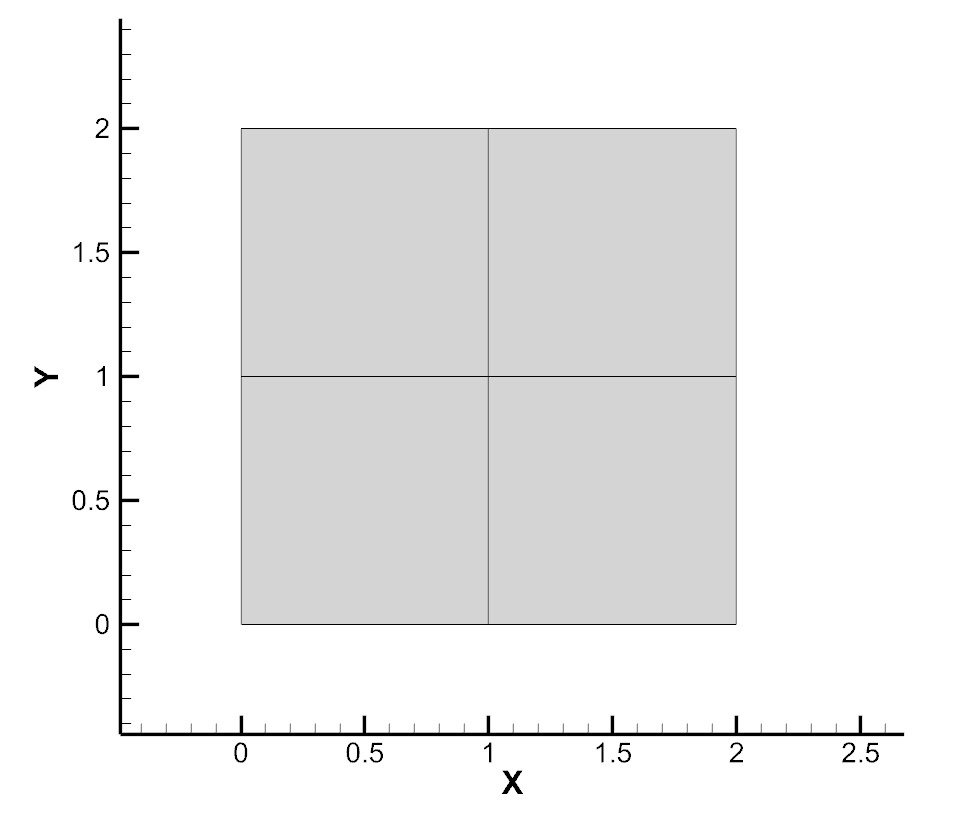
\includegraphics[width=0.6\textwidth]{2d.png}
  \caption{2D网格示例}
  \label{2dMesh}
\end{figure}

\begin{lstlisting}
  (0 " Created by : Fluent_V6 Interface Vers. 18.2.0") % 版本信息
  (2 2) ---------------------------------------------- % 维度
  (0 "Node Section") --------------------------------- % Nodes描述字段
  (10 (0 1 9 0 2)) ----------------------------------- % Nodes总述字段
  (10 (5 1 9 1 2) ------------------------------------ % Nodes头文字段
  (0 0
  1 0
  0 1
  1 1
  0 2
  1 2
  2 0
  2 1
  2 2))
  (12 (0 1 4 0 0)) ----------------------------------- % Cells总述字段
  (12 (6 1 4 1 3)) ----------------------------------- % Cells头文字段
  (13 (0 1 c 0 0)) ----------------------------------- % Faces总述字段
  (0 "Interior faces of zone FLUID") ----------------- % 内部面描述字段
  (13 (7 1 4 2 2)( ----------------------------------- % 内部Faces头文字段
  2 4 1 3
  4 3 1 2
  4 6 2 4
  8 4 3 4))
  (0 "Faces of zone FAR") ---------------------------- % "far"面描述字段
  (13 (8 5 c 9 2)( ----------------------------------- % "far"Faces头文字段
  1 2 1 0
  2 7 3 0
  3 1 1 0
  5 3 2 0
  7 8 3 0
  8 9 4 0
  6 5 2 0
  9 6 4 0))
  (0 "Zone Sections") -------------------------------- % Zone描述字段
  (39 (6 fluid FLUID)())
  (39 (7 interior int_FLUID)())
  (39 (8 pressure-far-field FAR)()) 
\end{lstlisting}

\subsection{3D ASCII文件示例}

3D文件的格式与2D相同,这里供保留部分内容做对比。网格以 $2\times2\times2$ 立方体为例,边长为2,其形状如图 \ref{3dMesh} 所示:
\begin{figure}[!htb]
  \centering
  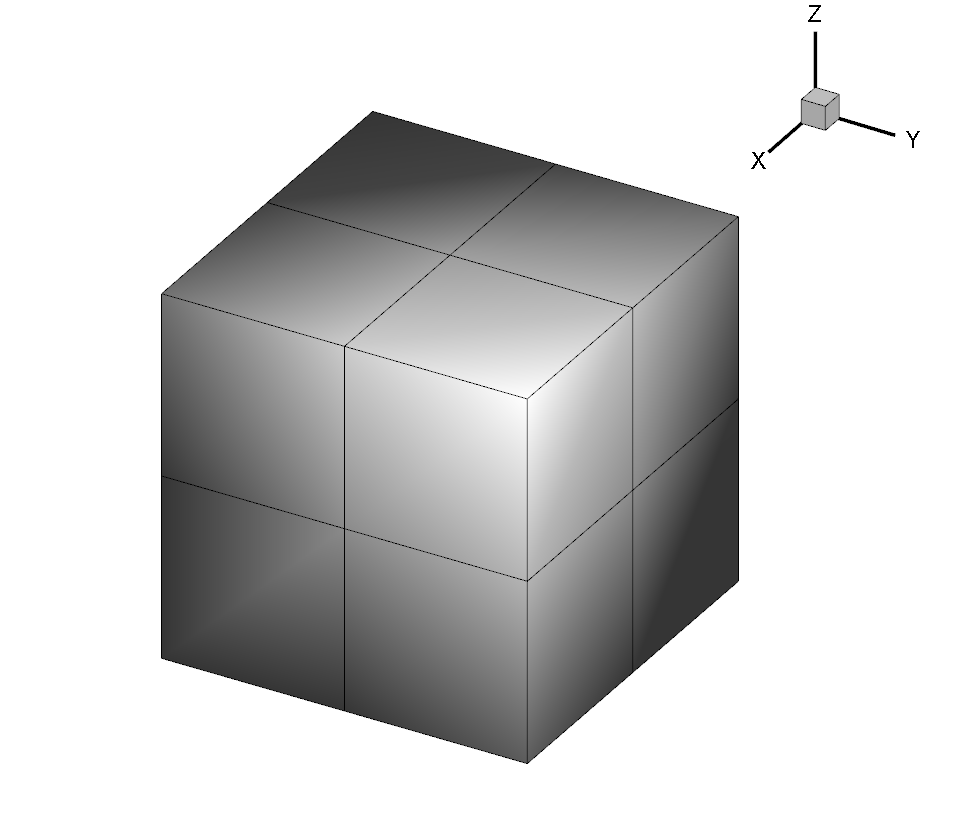
\includegraphics[width=0.6\textwidth]{3d.png}
  \caption{3D网格示例}
  \label{3dMesh}
\end{figure}

\begin{lstlisting}
  (0 " Created by : Fluent_V6 Interface Vers. 18.2.0")
  (2 3)
  (0 "Node Section")
  (10 (0 1 1b 0 3))
  (10 (5 1 1b 1 3)(0 0 0 1 0 0...))
  (12 (0 1 8 0 0))
  (12 (6 1 8 1 4))
  (13 (0 1 24 0 0))
  (0 "Interior faces of zone FLUID")
  (13 (7 1 c 2 4)(3 4 8 7 1 3 2 6 8 4 1 5...))
  (0 "Faces of zone FAR")
  (13 (1 d 24 9 4)(1 3 7 5 1 0 5 7 b 9 2 0...))
  (0 "Zone Sections")
  (39 (6 fluid FLUID)())
  (39 (7 interior int_FLUID)())
  (39 (1 pressure-far-field FAR)()) ------------ %自定义索引号1
\end{lstlisting}

查看上方的例子后,可以总结的ASCII文件的特点,以及补充的特性说明:
\begin{enumerate}
  \item Fluent Mesh内容总是在成对"()"内存放,形式是:(指令标号+内容);
  \item (指令标号+内容)中的内容可以是"()"的list,list内容的排布规则见下文;
  \item 文档不要求特定位置的换行,即(0 0 1 0 0 1...)与2D例子Nodes的数据内容等价;也可参考3D例之中的写法理解;
  \item 文档使用的分隔符为空格(space)。
\end{enumerate}

若按内容分类可分为:
\begin{enumerate}
  \item \textbf{描述字段}:用来描述下方的内容,相当于注释\textcolor{red}{(可省略)};
  \item \textbf{总述字段}:用于对内容进行总述(相当于头文字段的总结),常见于node,cell信息等模块\textcolor{red}{(不可省略,且必须在对应的头文字段前)};
  \item \textbf{头文字段}:用于描述各部分的内容的类型,成员起止索引号,成员类型等信息\textcolor{red}{(不可省略)};
  \item \textbf{数据内容}:在相应的头文字段的"()"内,为网格各类模块的具体信息,包括node坐标,几何关系等内容\textcolor{red}{(不可省略)}。
\end{enumerate}


\section{Grid Sections}\label{GridSections}

\subsection{描述字段}\label{Comment}
\begin{lstlisting}
  {描述字段格式}:(0 "comment text")
  {格式解释}:0为指令标号;
             "comment text"为描述文本,用""包括。
  {实例}:(0 " Created by : Fluent_V6 Interface Vers. 18.2.0")
\end{lstlisting}

\subsection{维度}\label{Dimensions}
\begin{lstlisting}
  {维度格式}:(2 n)
  {格式解释}:2为指令标号;
             第二个数字为维数,2表示2维、3表示3维。
  {实例}:(2 2); (2 3)
\end{lstlisting}

\subsection{Nodes 节点}\label{Nodes}
\begin{lstlisting}
  {node格式}:(10 (zone-id first-index last-index type ND)(x1 y1 z1 x2 y2 z2... ))
  {格式解释}:10为指令标号;
             zone-id为区域索引号;
             first-index为该区域第一个成员的索引号;
             last-index为该区域最后一个成员的索引号;
             type为node类型;
             ND为维度;
             (x y z)为每个node的坐标(10进制,Cartesian)。
  {实例}:(10 (0 1 9 0 2)); (10 (5 1 9 1 2)(0 0 1 0 0 1....))
\end{lstlisting}

\subsubsection{使用说明}
\begin{enumerate}
  \item \textbf{如果zone-id = 0}:first-index = 1,last-index为node总数,type置0,ND后面不跟坐标数据。此时相当于对nodes的整体说明,即总述字段;
  \item \textbf{如果zone-id > 0}:表示结构体中的nodes属于索引号zone-id的zone区域。此时first-index和last-index为该zone区域的node起止索引号,node的坐标信息在ND后的()内;
  \item \textbf{如果ND = 2}:表示2维,node数据不包含z坐标。
\end{enumerate}

\subsubsection{type设置规则}\label{node-type}
\begin{enumerate}
  \item[-] \lstinline{0}: "virtual" nodes -- 虚拟节点;
  \item[-] \lstinline{1}: no(any) type -- 通用型;
  \item[-] \lstinline{2}: boundary nodes -- 边界节点。
\end{enumerate}

\subsection{Cells 单元}\label{Cells}
\begin{lstlisting}
  {cell格式}:(12 (zone-id first-index last-index type element-type)())
  {格式解释}:12为指令标号;
             zone-id为区域索引号;
             first-index为该区域第一个成员的索引号;
             last-index为该区域最后一个成员的索引号;
             type为cell物理属性;
             element-type为cell类型;
             ()仅当element-type = 0时使用。
  {实例}:(12 (0 1 4 0 0)); (12 (6 1 4 1 3))
\end{lstlisting}

\subsubsection{使用说明}
\begin{enumerate}
  \item \textbf{如果zone-id = 0}:first-index = 1,last-index为cell总数(若last-index = 0则表示文件中无cell),
                                  type置0(计算时Fluent会忽略type = 0的区域(f非激活区)),element-type不显示(或置0)。此时相当于对cells的整体说明,即总述字段;
  \item \textbf{如果zone-id > 0}:表示结构体中的cells属于索引号zone-id的zone区域。type = 1 为流体,type = 20为Cell Tree;
  \item cell中没有显示表示出其包含的faces与nodes信息,但可通过点、面、单元关系格式\ref{nodefacecell}间接确定。
\end{enumerate}
~\\
\textbf{特别注意}:如果cell类型为混合型(element-type = 0),则列出每个cell的类型。此时cell格式后接一对()。
具体可见下面的例子,区域9有61个cell,其中前3个为三角cell,紧接两个四边形cell,等等。
\begin{lstlisting}
  (12 (9 1 3d 1 0)(
  1 1 1 3 3 1 1 3 1 ...))
\end{lstlisting}

\subsubsection{element-type设置规则}\label{element-type}
\begin{enumerate}
  \item[-] \lstinline{0}: mixed -- 混合型;
  \item[-] \lstinline{1}: triangular -- 三角形;
  \item[-] \lstinline{2}: tetrahedral -- 四面体;
  \item[-] \lstinline{3}: quadrilateral -- 四边形;
  \item[-] \lstinline{4}: hexahedral -- 六面体;
  \item[-] \lstinline{5}: pyramid -- 四棱锥(金字塔);
  \item[-] \lstinline{6}: wedge -- 楔形;
  \item[-] \lstinline{7}: polyhedral -- 多面体。
\end{enumerate}

\begin{figure}[!htb]
  \centering
  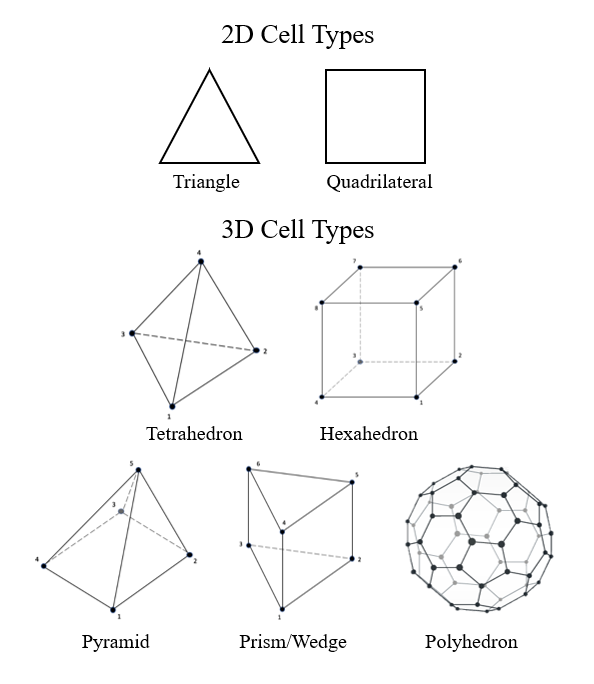
\includegraphics[width=0.5\textwidth]{elementtype.png}
  \caption{element-type展示}
  \label{elementtype}
\end{figure}

\subsection{Faces 面}\label{Faces}
\begin{lstlisting}
  {face格式}:(13 (zone-id first-index last-index bc-type face-type)())
  {格式解释}:13为指令标号;
             zone-id为区域索引号;
             first-index为该区域第一个成员的索引号;
             last-index为该区域最后一个成员的索引号;
             bc-type为边界条件;
             face-type为face类型;
             ()内存放node、face、cell的关系。
  {实例}:(13 (0 1 c 0 0)); (13 (7 1 4 2 2)(2 4 1 3 4 3 1 2...))
\end{lstlisting}

\subsubsection{使用说明}
\begin{enumerate}
  \item \textbf{如果zone-id = 0}:first-index = 1,last-index为face总数,bc-type不显示(或置0)。此时相当于对faces的整体说明,即总述字段;
  \item \textbf{如果zone-id > 0}:表示结构体中的faces属于索引号zone-id的zone区域,face数据的信息在随后的()内。
\end{enumerate}

\subsubsection{bc-type设置及介绍(标号采用16进制)}\label{bc-type}
\begin{enumerate}
  \item[-] \textcolor{blue}{\lstinline{2(Ox2)}: interior -- 内部边界};
  \item[-] \textcolor{blue}{\lstinline{3(Ox3)}: wall -- 壁面};
  \item[] 壁面 -- 粘性计算中默认为无滑移条件。当壁面存在运动时,可定义切向速度作为边界条件,或者定义剪切应力作为边界条件。壁面可以为双侧壁面(两个流体区域的交界面),
  即作为边界的face的两个相邻cells(c0 c1)可以同时存在。
  \item[-] \textcolor{red}{\lstinline{4(Ox4)}: pressure-inlet, inlet-vent, intake-fan -- 压力进口、通风进口、进口风扇边界};
  \item[] 1、压力进口边界 -- 可以理解为是没有遮挡的进口边界。界面可用于不可压缩和可压缩流动。当进口压强已知,而流动速度或流量未知时,可使用压力进口边界。
  压力进口条件也可用于定义外部或非受限流动的“自由边界”。
  \item[] 2、通风进口条件 -- 可以理解为是界面上被均匀遮挡的进口边界。通过给定损失系数、流动方向、环境压强和温度定义流场进口处的边界条件。
  \item[] 3、进口风扇边界 -- 可以用压强跃升、流动方向、环境压强和温度等参数的集合作为进口风扇简化模型的进口边界。
  \item[-] \textcolor{red}{\lstinline{5(Ox5)}: pressure-outlet, outlet-vent, exhaust-fan -- 压力出口、通风出口、排气风扇边界};
  \item[] 1、压力出口边界 -- 压力出口边界在流场出口边界上定义静压,而静压的值仅在流场为亚音速时使用。如果在出口边界上流场达到超音速,则边界上的压强将从流场内部插值得到。
  在压力出口边界上还需定义“回流(Backflow)”条件,用于处理出现回流时的边界边界条件。
  \item[] 2、通风出口 -- 用于模拟具有指定损失系数和环境(排放)静压和温度的通风出口。
  \item[] 3、排气风扇边界 -- 用于模拟具有指定压力跃变和环境(排放)静压的排气扇。
  \item[-] \textcolor{red}{\lstinline{7(Ox7)}: symmetry -- 对称边界};
  \item[] 对称边界 -- 流场中的流动及边界形状具有镜像对称性时,可设置对称边界条件。对称面上法向速度为零、变量的法向梯度为零,其本质为零通量面。
  这种条件也可以用于定义粘性流动中的零剪切力滑移壁面。
  \item[-] \textcolor{red}{\lstinline{8(Ox8)}: periodic-shadow};
  \item[-] \textcolor{red}{\lstinline{9(Ox9)}: pressure-far-field -- 压力远场};
  \item[] 压力远场 -- 用于设定无限远处的自由边界条件,主要设置项目为自有流马赫数和静参数条件。采用压力远场时要求密度用理想气体假设计算,同时为满足“无限远”要求,计算边界应远离物面。
  \item[-] \textcolor{red}{\lstinline{10(Oxa)}: velocity-inlet -- 速度进口};
  \item[] 速度进口边界 -- 用进口处流场速度及相关流动变量作为边界条件。应注意,速度进口条件仅适用于不可压流,此外不要让速度进口条件过于靠近固体障碍物。
  \item[-] \textcolor{red}{\lstinline{12(Oxc)}: periodic -- 周期边界};
  \item[] 周期边界 -- 流场的边界形状和流场结构存在周期性变化时,可采用周期性边界条件。
  \item[-] \textcolor{blue}{\lstinline{14(Oxe)}: fan, porous-jump, radiator -- 风扇、多孔跃升边界、散热器};
  \item[] 1、风扇 -- 通过已知的风扇几何与流动特性模化的边界。可用于计算通过风扇的流量。
  \item[] 2、多孔跃升边界 -- 在已知一个肋板前后的速度或压强的增量时,可用多孔跃升边界定义这个肋板。与多孔介质模型相比,该模型更简单,稳定性及收敛性更好。
  在计算过滤器、薄肋板等内部边界时应采用这种边界条件。
  \item[] 3、散热器 -- 将压降系数和热交换系数作为散热器法向速度的函数定义边界模型。可用于计算换热器件的流场。
  \item[-] \textcolor{red}{\lstinline{20(Ox14)}: mass-flow-inlet -- 质量流量进口};
  \item[] 质量流量进口 -- 已知流场进口处的流量时,可以通过定义质量流量或质量通量的形式定义边界条件。如果流场在进口处的主要流动特征是质量流量保持不变,则适合采用质量流量进口。
  但是,因为流场进口总压变化将影响计算稳定性,应尽量回避使用质量流量进口条件。
  \item[-] \textcolor{blue}{\lstinline{24(Ox18)}: Interface -- 交界面};
  \item[] 交界面 -- 用来定义相接触的不同区域的接触面,成对出现。
  \item[-] \textcolor{blue}{\lstinline{31(Ox1f)}: parent -- hanging nodes父级};
  \item[] parent -- 当网格出现hanging nodes时要定义给其父级的边界条件。
  \item[-] \textcolor{red}{\lstinline{36(Ox24)}: outflow -- 出流};
  \item[] 出流边界 -- 在流场求解前,出口的流速和压强未知,可以使用出流边界条件。但不适用于可压缩流(密度变化)、存在压力进口的情况。
  \item[-] \textcolor{red}{\lstinline{37(Ox25)}: axis -- 轴};
  \item[] 轴 -- 在轴对称流场的对称轴(对称几何的中心线)上使用的边界条件,使用时注意于对称边界区分。
\end{enumerate}
\textbf{注:\textcolor{blue}{蓝色}为内部面边界;\textcolor{red}{红色}为外部面边界。}

\subsubsection{face-type设置规则}\label{face-type}
\begin{enumerate}
  \item[-] \lstinline{0}: mixed -- 混合型;
  \item[-] \lstinline{2}: linear -- 线段(2D);
  \item[-] \lstinline{3}: triangular -- 三角形;
  \item[-] \lstinline{4}: quadrilateral -- 四边形;
  \item[-] \lstinline{5}: polygonal -- 多边形。
\end{enumerate}

具体的face-type形状可参考下图:
\begin{figure}[!htb]
  \centering
  
\includegraphics[width=0.6\textwidth]{facetype.png}
  \caption{face-type展示}
  \label{facetype}
\end{figure}

\subsubsection{点、面、单元关系格式}\label{nodefacecell}
\begin{lstlisting}
  {关系格式}:(n0 n1 n2 c0 c1)
  {格式解释}:n*(n0、n1、n2...)表示node索引号,其最大数量与face-type相关;
             c*(c0、c1)表示face两侧的cell索引号;
\end{lstlisting}

face包含的nodes按逆(顺)时针顺序排列,按其顺序连接的线段路径不能有交叉。

对于3D情况,c0索引号按node排序由右手定则的方向确定,c1则在face的另一边,如图\ref{3dc0c1}。
该例子的文本为((4) 1 2 6 5 c0 c1)其中“(4)”代表face包含的nodes数,但仅在face-type = 0或5时使用;
\begin{figure}[!htb]
  \centering
  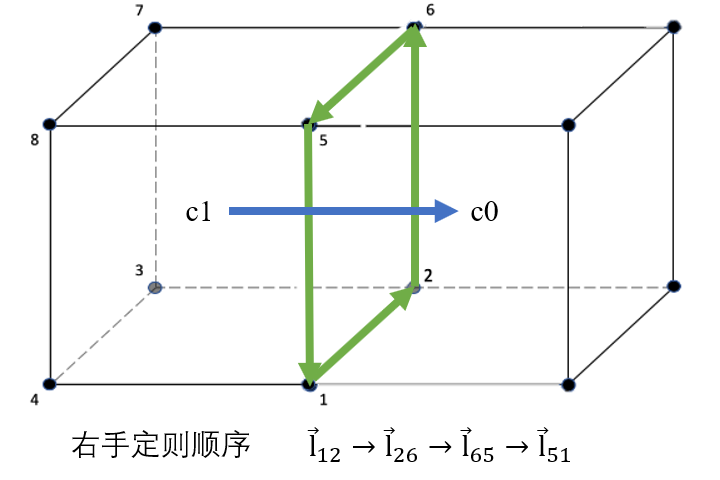
\includegraphics[width=0.55\textwidth]{3dc0c1.png}
  \caption{3D网格中c0索引号}
  \label{3dc0c1}
\end{figure}

对于2D情况,设一个指向平面外的$\overrightarrow{k}$,则$\overrightarrow{k}\times\overrightarrow{r}$的方向指向c0,另一边为c1,如图\ref{2dc0c1};
该例子的文本为((2) 1 2 c0 c1)其中“(2)”代表face包含的nodes数,但仅在face-type = 0或5时使用;
\begin{figure}[!htb]
  \centering
  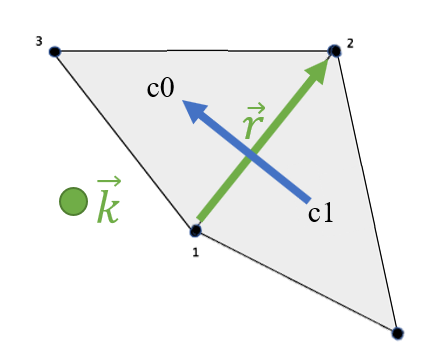
\includegraphics[width=0.4\textwidth]{2dc0c1.png}
  \caption{2D网格中c0索引号}
  \label{2dc0c1}
\end{figure}

在边界处一般通过调整node排序使c1为0,即保证c0一直存在。

当网格为混合类型(face-type = 0)或多边形类型(face-type = 5),每一行说明face的语句应以node数目开头:
\begin{lstlisting}
  (x n0 n1 ... nf c0 c1) 
  {实例}:五边形(... 5 89 8a 12 f 5 12 4 ...) 
\end{lstlisting}

\subsection{Face Tree}\label{Face-Tree}
\begin{lstlisting}
  {Face Tree格式}:(59 (face-id0 face-id1 parent-zone-id child-zone-id)
                 (number-of-kids kid-id-0 kid-id-1 ... kid-id-n))
  {格式解释}:59为指令标号;
             face-id0为区域第一个父级face的索引号;
             face-id1为区域最后一个父级face的索引号;
             parent-zone-id为父级face所在区域id;
             child-zone-id为子级face所在区域id;
             number-of-kids为子级face的数量;
             kid-id-n为子级face的索引号。
  {实例}: (59 (139 13a 5 9)(2 135 136 2 137 138))
\end{lstlisting}
该部分的详细网格实例可参考 \ref{Cartesianmesh}。

\subsection{Cell Tree}\label{Cell-Tree}
\begin{lstlisting}
  {Cell Tree格式}:(58 (cell-id0 cell-id1 parent-zone-id child-zone-id)
                 (number-of-kids kid-id-0 kid-id-1 ... kid-id-n))
  {格式解释}:58为指令标号;
             cell-id0为区域第一个父级cell的索引号;
             cell-id1为区域最后一个父级cell的索引号;
             parent-zone-id为父级cell所在区域id;
             child-zone-id为子级cell所在区域id;
             number-of-kids为子级cell的数量;
             kid-id-n为子级cell的索引号。
  {实例}:(58 (8d 92 2 6)(4 75 76 77 78 4 79 7a 7b 7c ...))            
\end{lstlisting}
该部分的详细网格实例可参考 \ref{Cartesianmesh}。


\section{Non-Grid Sections}\label{NonGridSections}

\subsection{Zone 区域}\label{Zone}
\begin{lstlisting}
  {区域格式}:(39/45 (zone-id zone-type zone-name domain-id)())
  {格式解释}:39/45为指令标号;
             zone-id为区域索引号(10进制);
             zone-type为区域类型(一般是指边界条件);
             zone-name为区域名称;
             domain-id用于关联边界条件与相(整型);
             ()空。
  {实例}:(39 (8 pressure-far-field FAR)())
\end{lstlisting}

\textbf{需要注意的事项:}
\begin{enumerate}
  \item 头文字段最后的空"()"必须存在,这部分内容由Fluent求解器填写;
  \item 当zone内容只有zone-id, zone-type, zone-name, 和domain-id时推荐指令标号45;
  \item 当有边界条件时指令标号必须用39。
\end{enumerate}

\subsubsection{zone-type设置规则}\label{zone-type}
\begin{table}[!htb]
  \centering
  \caption{可用的zone-type种类}
  \begin{tabular}{*{3}{l}}
   \hline
   \texttt{degassing}       & \texttt{exhaust-fan}   & \texttt{fan} \\
   \texttt{fluid}           & \texttt{geometry}      & \texttt{inlet-vent} \\
   \texttt{intake-fan}      & \texttt{interface}     & \texttt{interior} \\
   \texttt{internal}        & \texttt{mass-flow-inlet}          & \texttt{outflow} \\
   \texttt{outlet-vent}     & \texttt{parent-face}   & \texttt{porous-jump} \\
   \texttt{pressure-far-field}         & \texttt{pressure-inlet}     & \texttt{pressure-outlet} \\
   \texttt{radiator}        & \texttt{solid}         & \texttt{symmetry} \\
   \texttt{velocity-inlet}  & \texttt{wall}          & \texttt{wrapper} \\
   \hline
  \end{tabular}
\end{table}


\section{复杂情况的网格实例}

\subsection{Cartesian mesh}\label{Cartesianmesh}

这里解释的Cartesian mesh是基于树形数据结构的笛卡尔网格,这种网格的特点之一是含有Hanging Node。
Hanging Node指的是拓扑结构不完备的Node,如图\ref{hangingnode}左中圈出的Node不属于其下方的三角形;与之相对的是右中展示的网格,该网格中不含有Hanging Node。

目前,Cartesian mesh常用于AMR(Adaptive Mesh Refinement)自适应网格方法中的网格重构,以及对复杂曲面的边界加密或跟踪。
主流的CFD求解器都有相应Cartesian mesh生成方法(如Fluent Meshing的CutCell网格生成器、STAR CCM+的Trimmed Mesher网格生成器、
以及OpenFOAM的SnppyHexMesh网格生成器)。
\begin{figure}[!htb]
  \centering
  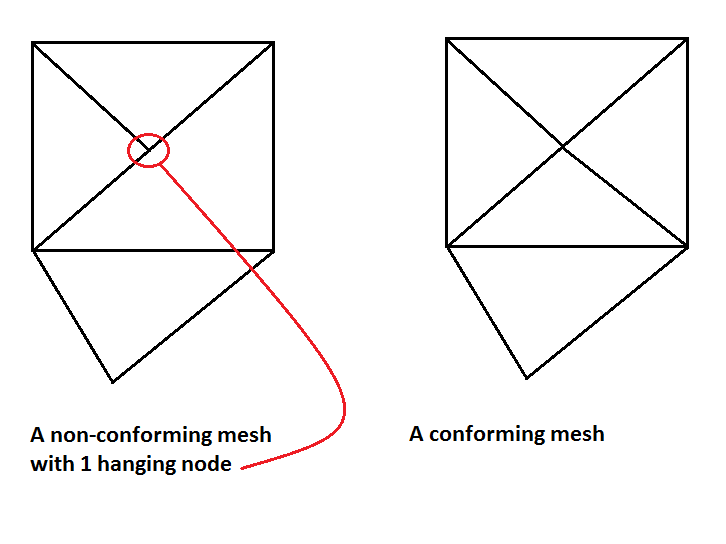
\includegraphics[width=0.6\textwidth]{hangingnode.png}
  \caption{Hanging Node示例}
  \label{hangingnode}
\end{figure}

在Fluent求解器中Haning Nodes由Face Tree、Cell Tree控制,这两个区域描述的内容类似树形结构(Tree)的节点,一层层嵌入网格信息。
这里采用Fluent Mesh中树形Cartesian mesh结构,给出一层Tree结构的网格实例(多层结构类似)。
可参考Face Tree \ref{Face-Tree},及Cell Tree \ref{Cell-Tree}理解相应内容,由于Nodes、Faces、cells都在图中一一标明,
相应内容不再赘述,这个实例的关注点在Face Tree和Cell Tree的结构上。具体可参考图 \ref{cartesianmeshdetal}。 
\begin{figure}[!htb]
  \centering
  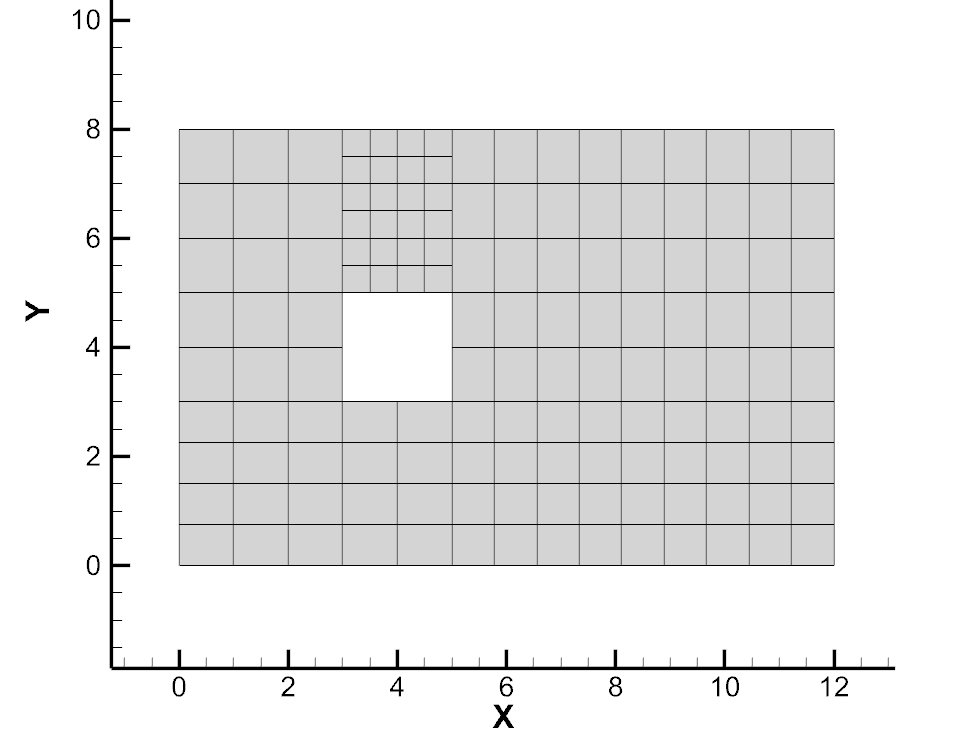
\includegraphics[width=0.45\textwidth]{cartesianmesh.png}
  \caption{树形数据结构Cartesian mesh示例}
  \label{cartesianmeshexample}
\end{figure}

\begin{lstlisting}
  (0 "Grid:")
  (12 (0 1 92 0))
  (13 (0 1 149 0))
  (10 (0 1 ac 0 2))
  (12 (6 1 8c 1 3))
  (12 (2 8d 92 20 3)) -------------- % Cell的type为20,表示parent-cell
  (58 (8d 92 2 6) ------------------ % Cell Tree 其内容可理解为树形结构中节点的概念
  (4 75 76 77 78
   4 79 7a 7b 7c
   4 7d 7e 7f 80
   4 81 82 83 84
   4 85 86 87 88
   4 89 8a 8b 8c))
  (13 (7 1 fe 2 2)(1 2 1 5 2 3 1 2 2 4 2 6 4 5 2 3 ...))
  (13 (8 ff 12e 9 2)(a9 1 1 0 3 a9 1 0 5 3 2 0 7 5 3 ...))
  (13 (9 12f 138 3 2)(13 1a 11 0 1a 1b 12 0 2a 13 1f 0 ...))
  (13 (5 139 13a 1f 2) ------------- % Face的bc-type为1f,表示parent-face,下同
  (1b 8c 8d 0
  8c 5f 90 0))
  (13 (4 13b 13c 1f 2)
  (99 9b 8f 0
  a6 99 92 0))
  (13 (3 13d 149 1f 2)
  (8c 8e 8d 90
  8e 24 8d 8e
  1b 24 19 8d
  8e 94 8e 91
  94 25 8e 8f
  24 25 1a 8e
  94 99 8f 92
  25 9b 1b 8f
  5f 71 90 5a
  71 8e 90 91
  71 73 91 5b
  73 94 91 92
  73 a6 92 5c))
  (59 (139 13a 5 9)
  (2 135 136
  2 137 138))
  (59 (13b 13c 4 8)
  (2 12b 12c
  2 12d 12e))
  (59 (13d 149 3 7)
  (2 cd ce
  2 cf d0
  2 d1 d2
  2 d7 d8
  2 d9 da
  2 db dc
  2 e1 e2
  2 e3 e4
  2 e9 ea
  2 eb ec
  2 f1 f2
  2 f3 f4
  2 f9 fa))
  (10 (1 1 ac 1 2)(1.0000000000000000e+00  0.0000000000000000e+00 ...))
  (39 (6 fluid fluid 1)())
  (39 (8 pressure-far-field far 1)())
  (39 (7 interior int_fluid 1)())
  (39 (9 wall wall 1)())
\end{lstlisting}

\begin{figure}[!htb]
  \centering
  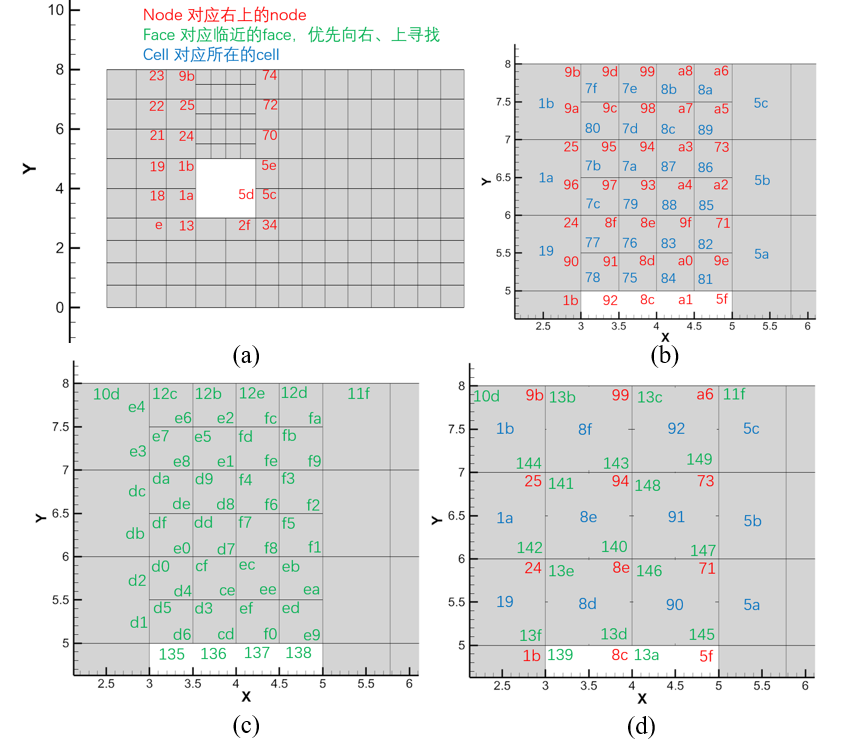
\includegraphics[width=0.75\textwidth]{cartesianmeshdetal.png}
  \caption{网格元素索引号图;(a)网格总体视图;(b)Tree区域的child-cells、nodes索引号;
                          (c)Tree区域的child-faces索引号;(d)Tree区域的parent-cells、faces、nodes索引号}
  \label{cartesianmeshdetal}
\end{figure}

\textbf{需要注意的事项:}
\begin{enumerate}
  \item 可参考图\ref{treestruct}的内容理解何为网格tree结构;
  \item Fluent中的Face、Cell Tree分别用来确定存在child-face、cell的Face和Cell,各层级间不允许跨越,各层的网格必须一层层排列。
        安全的做法就是一层一层写,不要考虑的很复杂;
  \item 通过静态网格生成器生成的网格可能缺失tree结构的信息。
\end{enumerate}

\begin{figure}[!htb]
  \centering
  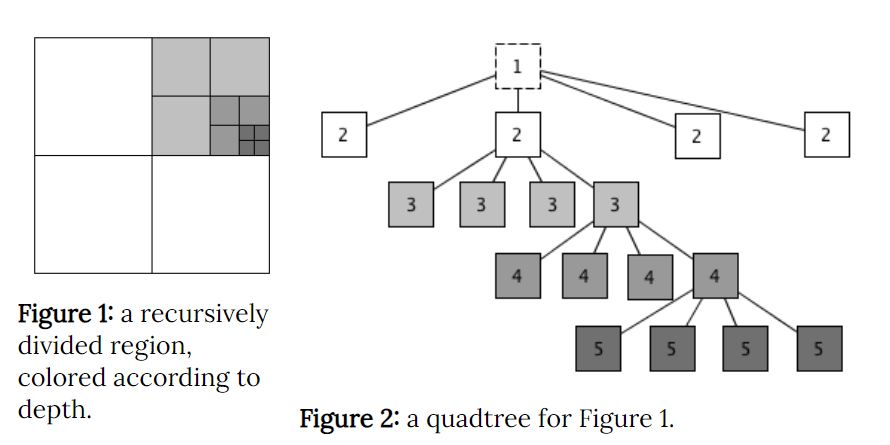
\includegraphics[width=0.7\textwidth]{treestruct.png}
  \caption{网格Tree结构说明图}
  \label{treestruct}
\end{figure}

\section{二进制文件说明}

Fluent Mesh的二进制文件与ASCII文件的区别非常小,要说明的是二进制文件除了数据内容外的内容都按ASCII解码。
下面是一段二进制文件的实例。

\begin{lstlisting}
  {实例}:(3013 (7 d 10 5 4)(二进制数据内容)End of Binary Section 3013)
\end{lstlisting}

需要说明的事项:
\begin{enumerate}
  \item 二进制文件中除数据内容外均按ASCII存储;
  \item 对于有数据内容的区域,二进制的头文字段与ASCII文件相比,指令标号增加两个拓展位(20为单精度;30为双精度)
  \item 二进制文件的数据以二进制存储,每个数据占用的字节数由指令标号添加的拓展位确定,数据间不需要分隔;
  \item 二进制数据结尾以指定的字符串标识"End of Binary Section xxxx"。
\end{enumerate}
\textcolor{red}{注:Cell区域有时数据为空(不等于无数据,空就是数据),也要按二进制文件格式在结尾添加指定的字符串标识。}


\section{附录}

\subsection{指令标号检索}\label{index}
检索列表列出Fluent Mesh文件网格内容的所有可用的指令标号,后接-optional的代表可选项目;后接-required的代表必需项目或依照相应条件的必需项目。
\begin{enumerate}
  \item[-] \lstinline{0}: Comment\upref{Comment}, -optional;
  \item[-] \lstinline{1}: Header, -optional;
  \item[-] \lstinline{2}: Dimensions\upref{Dimensions}, -optional;
  \item[-] \lstinline{10}: Nodes\upref{Nodes}, -required;
  \item[-] \lstinline{11}: Edges, -optional;
  \item[-] \lstinline{12}: Cells\upref{Cells}, -required;
  \item[-] \lstinline{13}: Faces\upref{Faces}, -required;
  \item[-] \lstinline{18}: Periodic Shadow Faces, -required with periodic boundaries;
  \item[-] \lstinline{39 or 45}: Zone\upref{Zone}, -required;(当有边界条件时必须用39)
  \item[-] \lstinline{58}: Cell Tree\upref{Cell-Tree}, -required only for grids with hanging-node adaption;
  \item[-] \lstinline{59}: Face Tree\upref{Face-Tree}, -required only for grids with hanging-node adaption;
  \item[-] \lstinline{61}: Interface Face Parents, -required only for grids with non-conformal Interfaces.
\end{enumerate}

\subsection{X-type设置检索}
该部分包含文档中出现的各种type,可用来速查。
\begin{enumerate}
  \item node-type\upref{node-type};
  \item element-type\upref{element-type};
  \item bc-type\upref{bc-type};
  \item face-type\upref{face-type};
  \item zone-type\upref{zone-type}.
\end{enumerate}

\subsection{文档资源}
本文档PDF版本使用\LaTeX{}编写。如果需要文档的源码、图片资源请到GitHub项目页面
\url{https://github.com/iforever-yh/Fluent-mesh-format}
下载。

\end{document}